\documentclass{article}
\usepackage{graphicx} % Required for inserting images
\usepackage[utf8]{inputenc}
\usepackage{lmodern}
\usepackage{amsmath}
\usepackage{hyperref}
\usepackage{enumitem}
\usepackage{cite}
\usepackage{tabularx}

\title{Traffic Obfuscation in Libvirt-Based Virtualized Networks}
\author{Kleiton Pereira}
\date{Feb 2025}

\begin{document}

\maketitle

\begin{abstract}
This report explores the use of libvirt in managing virtualized networks and investigates strategies for implementing traffic obfuscation at two levels: as packets leave the virtual machine (VM) and as they exit the host machine. We examine encryption-based obfuscation methods, as well as alternative approaches such as traffic shaping, tunneling, and padding. We also discuss performance overhead in terms of latency, throughput, and computational cost, and provide implementation recommendations and future research directions.
\end{abstract}

\section{Introduction}
The growing need for privacy in network communications has led to research into methods of traffic obfuscation. In virtualized environments managed by libvirt, it is possible to apply obfuscation both at the VM level and at the host egress. This report outlines the architecture of libvirt, reviews potential obfuscation strategies, analyzes their performance overhead, and provides implementation recommendations and research directions. 

\section{Overview of Libvirt}
Libvirt is an open-source API, daemon, and management toolkit that abstracts the complexities of platform virtualization, providing a uniform interface for managing various hypervisors such as KVM, Xen, and VMware \cite{libvirt2013}. Key aspects of libvirt include:
\begin{itemize}[noitemsep]
    \item \textbf{VM Lifecycle Management:} Starting, stopping, and migrating VMs.
    \item \textbf{Virtual Network Management:} Creating and managing virtual networks (e.g., NAT, bridged, isolated) and the associated components such as Linux bridges and tap devices.
    \item \textbf{Network Filters:} Enforcing security policies using NWFilter, which provides anti-spoofing and traffic control mechanisms.
\end{itemize}

In typical setups, libvirt creates a default virtual network (e.g., a Linux bridge like \texttt{virbr0}) that handles IP address management via DHCP (often using \texttt{dnsmasq}) and NAT for outbound traffic. This environment sets the stage for implementing additional traffic obfuscation strategies.

\begin{figure}[h]
\caption{Libvirt high-level structure.}
\centering
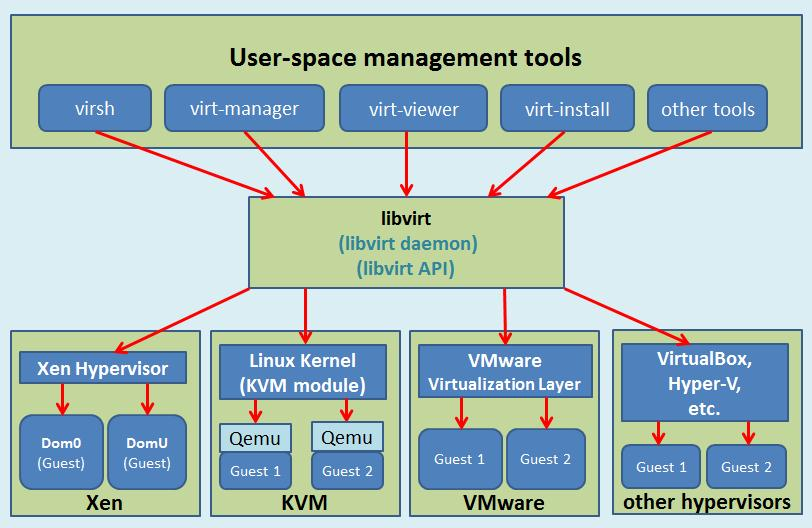
\includegraphics[width=0.9\textwidth]{libvirt.png}
\end{figure}

\section{Traffic Obfuscation Strategies in Libvirt-Based Networks}
In the context of libvirt-managed environments, two potential points for traffic obfuscation are identified:
\begin{enumerate}[label=\arabic*.]
    \item \textbf{Obfuscation at the VM Egress:} As packets leave the VM via its virtual NIC, they pass through libvirt’s virtual networking layer. Here, obfuscation can be implemented by leveraging libvirt’s network filter (NWFilter) framework or by routing traffic through a custom user-space service. This approach ensures that the traffic is obfuscated even within the host and is often implemented per-VM.
    \item \textbf{Obfuscation at the Host Egress:} Alternatively, traffic can be obfuscated as it leaves the host machine. Techniques here involve using system-level tools such as iptables, \texttt{tc}, or Open vSwitch to tunnel or shape the traffic. A centralized obfuscation module on the host can encrypt and pad traffic before it is sent to the external network.
\end{enumerate}

\subsection{Encryption-Based Obfuscation}
Encryption is a primary method to achieve confidentiality. By encrypting the payload, the contents become indecipherable even though packet metadata may remain visible. Common approaches include:
\begin{itemize}[noitemsep]
    \item \textbf{Application-Layer Encryption:} Protocols like TLS/SSL are employed at the application level.
    \item \textbf{Network-Layer Encryption:} Implementations such as IPsec or VPN tunnels (e.g., WireGuard, OpenVPN) on the host or within the VM.
\end{itemize}
While encryption hides payload contents, side-channel features (such as packet sizes and timing) may still leak information.

\subsection{Alternative Methods: Traffic Shaping, Tunneling, and Padding}
Beyond encryption, other techniques can be applied:
\begin{itemize}[noitemsep]
    \item \textbf{Traffic Shaping:} Adjusting packet timing to create a constant bitrate or to add random delays. This approach helps to mask burst patterns.
    \item \textbf{Tunneling:} Encapsulating traffic within a different protocol (e.g., HTTP/HTTPS or GRE/VXLAN) to hide the original traffic signatures.
    \item \textbf{Padding and Chaff:} Adding random padding to packets or injecting dummy traffic to equalize packet sizes and obscure communication patterns.
\end{itemize}

Table~\ref{tab:methods} summarizes the advantages and disadvantages of the various approaches.

\begin{table}[ht]
\centering
\begin{tabularx}{\linewidth}{|p{2.5cm}|X|X|}
\hline
\textbf{Approach} & \textbf{Advantages} & \textbf{Disadvantages} \\
\hline
\textbf{VM Egress (Hypervisor-level)} & 
\begin{itemize}[leftmargin=*,noitemsep]
    \item Enforced outside the VM; transparent to the user.
    \item Per-VM granularity.
\end{itemize} & 
\begin{itemize}[leftmargin=*,noitemsep]
    \item Limited by libvirt’s native filtering capabilities.
    \item May require custom development.
    \item Potential per-packet processing overhead.
\end{itemize} \\
\hline
\textbf{Host Egress} & 
\begin{itemize}[leftmargin=*,noitemsep]
    \item Centralized control and easier management.
    \item Leverages host hardware acceleration.
    \item Aggregated cover traffic across multiple VMs.
\end{itemize} & 
\begin{itemize}[leftmargin=*,noitemsep]
    \item Traffic is exposed within the host before obfuscation.
    \item Single point of configuration for all VMs.
\end{itemize} \\
\hline
\textbf{Encryption (IPsec/VPN)} & 
\begin{itemize}[leftmargin=*,noitemsep]
    \item Strong confidentiality.
    \item Widely supported and can utilize hardware acceleration.
\end{itemize} & 
\begin{itemize}[leftmargin=*,noitemsep]
    \item Does not obscure metadata (sizes, timing).
    \item Additional processing overhead.
\end{itemize} \\
\hline
\textbf{Traffic Shaping} & 
\begin{itemize}[leftmargin=*,noitemsep]
    \item Masks timing patterns and burstiness.
    \item Can be tuned to mimic constant traffic.
\end{itemize} & 
\begin{itemize}[leftmargin=*,noitemsep]
    \item Introduces latency and jitter.
    \item May require sending dummy traffic.
\end{itemize} \\
\hline
\textbf{Padding \& Chaff} & 
\begin{itemize}[leftmargin=*,noitemsep]
    \item Obscures packet size information.
    \item Confuses size-based traffic analysis.
\end{itemize} & 
\begin{itemize}[leftmargin=*,noitemsep]
    \item High bandwidth overhead.
    \item Increases overall data volume.
\end{itemize} \\
\hline
\end{tabularx}
\caption{Comparison of Traffic Obfuscation Approaches}
\label{tab:methods}
\end{table}

\section{Performance Overhead Analysis}
Implementing obfuscation impacts several network performance metrics:
\begin{itemize}[noitemsep]
    \item \textbf{Latency:} Encryption introduces minimal latency (microseconds to a few milliseconds), whereas traffic shaping that adds deliberate delays can increase overall latency and jitter.
    \item \textbf{Throughput:} Overhead from dummy traffic and rate limiting can reduce effective throughput. For instance, padding schemes might significantly inflate the volume of transmitted data.
    \item \textbf{CPU and Resource Usage:} Both encryption and packet manipulation increase CPU utilization. In centralized host-level obfuscation, a single processing node might become a bottleneck.
\end{itemize}

Studies in the literature have shown trade-offs between privacy and performance \cite{paddingShaping2019}. Systems such as \emph{Ditto} demonstrate that, with hardware offloading, it is possible to achieve near line-rate performance even while applying heavy obfuscation \cite{ditto2021}.

\section{Implementation Recommendations}
Based on the strategies discussed, a hybrid approach that leverages both host-level and VM-level techniques is recommended. Below are some guidelines and a sample pseudocode snippet.

\subsection{Tools and Technologies}
\begin{itemize}[noitemsep]
    \item \textbf{Libvirt API:} Use Python or C bindings to manage VM interfaces and virtual networks.
    \item \textbf{Linux Networking Tools:} iptables/nftables for packet redirection, \texttt{tc} for traffic shaping, and Open vSwitch for advanced tunneling.
    \item \textbf{Encryption Tools:} Implement IPsec (using strongSwan or Libreswan) or VPN solutions like WireGuard.
    \item \textbf{Programming Libraries:} For prototyping, Python libraries such as \texttt{scapy} and \texttt{netfilterqueue} can be used. For performance-critical code, consider C or eBPF.
\end{itemize}

\subsection{Proof-of-Concept Pseudocode}
Below is an illustrative pseudocode example using Python and Scapy to intercept and obfuscate traffic:

\begin{verbatim}
from scapy.all import sniff, sendp, Raw
import os

def encrypt_data(data, key):
    # Placeholder: implement symmetric encryption (e.g., AES)
    return AES_encrypt(data, key)

def pad_data(data, target_length):
    pad_len = target_length - len(data)
    if pad_len > 0:
        data += os.urandom(pad_len)
    return data

KEY = b'some16bytekey!!'
FIXED_PACKET_SIZE = 1500

def obfuscate_packet(pkt):
    if pkt.haslayer(Raw):
        original_payload = bytes(pkt[Raw].load)
        encrypted_payload = encrypt_data(original_payload, KEY)
        padded_payload = pad_data(encrypted_payload, 
                                  len(encrypted_payload) + (FIXED_PACKET_SIZE - len(pkt)))
        pkt[Raw].load = padded_payload
        pkt.len = None
        pkt.chksum = None
    return pkt

sniff(iface="vnet0", store=False,
      prn=lambda packet: sendp(obfuscate_packet(packet), iface="eth0"))
\end{verbatim}

This code listens on the VM interface (\texttt{vnet0}), encrypts and pads the packet payload, then sends it out through the external interface (\texttt{eth0}). In practice, consider more robust error handling, support for various packet types, and performance optimizations.

\section{Future Research Directions}
Future work in this area can address several challenges:
\begin{itemize}[noitemsep]
    \item \textbf{Optimizing Privacy vs. Overhead:} Developing adaptive algorithms that maximize privacy while minimizing latency and bandwidth overhead \cite{futurePrivacy2022}.
    \item \textbf{Automated Obfuscation Tuning:} Leveraging machine learning to dynamically adjust obfuscation parameters.
    \item \textbf{Integration with SDN/NFV:} Coordinating obfuscation across distributed virtualized infrastructures.
    \item \textbf{Hardware Offloading:} Exploring the use of SmartNICs and programmable switches (e.g., via P4) to implement obfuscation with minimal CPU overhead \cite{ditto2021}.
    \item \textbf{Security Implications:} Balancing obfuscation with the need for network monitoring and intrusion detection.
\end{itemize}

\section{Conclusion}
This report has provided a detailed technical discussion on using libvirt for implementing traffic obfuscation in virtualized networks. We have reviewed both VM-level and host-level strategies, analyzed the performance implications of various techniques, and provided implementation recommendations along with a proof-of-concept example. Future research should focus on fine-tuning the trade-offs between privacy and performance while considering practical deployment scenarios in dynamic cloud environments.

\bibliographystyle{plain}
\bibliography{refs}

\end{document}
